\subsection{Schusspfadberechnung}
\label{sec:anfang_3}
Im Folgenden wird die Schusspfadberechnung erläutert. Mithilfe der nicht aussortierten Pfosten sowie der Chokepoints wird der letzte Teil des Algorithmus erklärt, der die Lösung der Aufgabe berechnet und konstruiert. Ziel dieser Berechnung ist es, einen Schuss zu finden, der alle relevanten Tore in der vorgegebenen Reihenfolge passiert.

Um diesen Teil des Algorithmus zu ermöglichen, wurden im Vorfeld die Reihenfolge der Tore überprüft, die \textit{lr-Konfiguration} aller Tore gefunden, die Längen- und Breitengrad-Isoklinen der Tore berechnet, die Chokepoints gefunden und nicht relevante Pfosten herausgefiltert. Für das finden einer Lösung muss nach mehreren wichtigen Pfosten gesucht werden. Wie diese Pfosten charakterisiert und gefunden werden, wird im nächsten Unterkapitel erläutert.


\newpage
\subsubsection{Stützpfosten} 
Neben den Chokepoints spielt die Bestimmung zusätzlicher Stützpfosten eine entscheidende Rolle. Stützpfosten sind Pfosten, auf denen ein möglicher Schusspfad liegen kann, sie sind essentiell zum Finden einer Lösung. Dabei wird zwischen zwei Arten von Stützpfosten unterschieden.

\paragraph{Hauptstützpfosten:}
Für alle linken und alle alle rechten Pfosten wird separat der Winkel berechnet, der sich zwischen der Verbindungslinie von $t_n$ links/rechts zu $t_0$ links/rechts und der Verbindungslinie zu dem betreffenden Pfosten ergibt. Der Pfosten mit dem kleinsten Winkel wird als Hauptstützpfosten definiert (\hyperref[fig:hauptpfosten]{Abb. 10}). Er fungiert als eine Art „Anti Chokepoint“, da er als erster kritischer Pfosten in der Schussbahn wirkt, wenn in Richtung „links oben“ geschossen wird. 

\begin{figure}[h]
\centering
\label{fig:hauptpfosten}
 \begin{tikzpicture}[scale=2]

  \coordinate (t0R) at (0,0);
  \coordinate (tnR) at (4,0);
  \coordinate (t0L) at (1,4);
  \coordinate (tnL) at (5,4);

  \draw[thick] (t0L) -- (t0R);
  \draw[thick] (tnL) -- (tnR);
  \node[above left] at (t0L) {\(t_0^l\)};
  \node[above right] at (tnL) {\(t_n^l\)};
  \node[below left] at (t0R) {\(t_0^r\)};
  \node[below right] at (tnR) {\(t_n^r\)};

  \draw[dashed, blue] (t0L) -- (tnL) node[midway, above] {\(ll\)};
  \draw[dashed, blue] (t0R) -- (tnR) node[midway, below] {\(rr\)};

  \coordinate (P) at (3,2.1);
  \filldraw[green!70!black] (P) circle (2pt) node[above left] {\(P\)};

  \draw[thick, ->] (tnL) -- (P);

\draw pic[draw, green!70!black, very thick, angle radius=1.5cm, angle eccentricity=1.5, text={"$\theta_P$"}] {angle = P--tnL--t0L};
  \node[green!70!black, very thick] at (5.7, 4.7) {\(\theta_P\)};

  \coordinate (CP_left) at (1,1.5);

  \coordinate (CP_right) at (3.4,1.7);
 
  \draw[ultra thick, blue] (t0L) -- (CP_left) -- (tnL);
  \draw[ultra thick, red] (t0R) -- (CP_right) -- (tnR);

  \filldraw[blue] (CP_left) circle (2pt) node[above left] {\(C_l\)};
  \filldraw[red] (CP_right) circle (2pt) node[above right] {\(C_r\)};
  
\end{tikzpicture}
    \caption{Berechnung von Hauptstützpfosten. Die Abbildung zeigt das Initialpolygon bestehend aus \(t_0\), \(t_n\), \(ll\) und \(rr\). Das Kanalpolygon ist durch die Chokepoints \(C_l\) und \(C_r\) vereinfacht dargestellt. Die Berechnung des Winkels \(\theta_P\) ist an einem Pfosten \(P\) beispielhaft dargestellt. Der Winkel \(\theta\) wird im Uhrzeigersinn von der Linie \(ll\) zu der Verbindungslinie von \(t^l_n\) nach \(P\) gemessen. Wenn \(\theta_P\) der größte Winkel von den linken Pfosten ist, ist \(P\) der linke Hauptstützpfosten.}
\end{figure}

\newpage

\paragraph{Untergeordnete Stützpfosten:}
Es gibt zwei linke und und zwei rechte untergeordnete Stützpfosten, jeweils einen für den Hauptstützpfosten und einen für den Chokepoint.
Für die Berechnung der zwei untergeordneten Stützpfosten (\hyperref[fig:unterpfosten]{Abb. 11}) werden für die linken Pfosten zusätzlich die zwei Winkel von $t_n$ rechts über den Chokepoint und über den Hauptstützpfosten zu den verbleibenden Pfosten berechnet. Die Pfosten, bei denen einer dieser Winkel am größten ist, werden als untergeordnete Stützpfosten bestimmt. Analog werden diese Berechnungen auch bei den rechten Pfosten vorgenommen. Der Pfad ausgehend von dem linken Chokepoint zu seinem untergeordneten Stützpfosten ist der flachste Pfad an allen linken Pfosten vorbei ausgehend von diesem Chokepoint. Das gilt auch für den Hauptstützpfosten und seinen untergeordneten Stützpfosten.

\begin{figure}[H]
\centering
\label{fig:unterpfosten}
 \begin{tikzpicture}[scale=2.5]

  \coordinate (t0R) at (0,0);
  \coordinate (tnR) at (4,0);
  \coordinate (t0L) at (1,4);
  \coordinate (tnL) at (5,4);

  \coordinate (CP_left) at (1,1.5);

  \coordinate (CP_right) at (3.4,1.7);

  \draw[thick] (t0L) -- (t0R);
  \draw[thick] (tnL) -- (tnR);
  \node[above left] at (t0L) {\(t_0^l\)};
  \node[above right] at (tnL) {\(t_n^l\)};
  \node[below left] at (t0R) {\(t_0^r\)};
  \node[below right] at (tnR) {\(t_n^r\)};

  \draw[dashed, blue] (t0L) -- (tnL) node[midway, above] {\(ll\)};
  \draw[dashed, blue] (t0R) -- (tnR) node[midway, below] {\(rr\)};

\coordinate (P) at (2,1.5);

  \draw[thick] (CP_left) -- (P);
  \draw[thick] (tnR) -- (CP_left);

    \filldraw[green!70!black] (P) circle (2pt) node[above left] {\(P\)};

  \draw[ultra thick, blue] (t0L) -- (CP_left) -- (tnL);
  \draw[ultra thick, red] (t0R) -- (CP_right) -- (tnR);

  \filldraw[blue] (CP_left) circle (2pt) node[above left] {\(C_l\)};
  \filldraw[red] (CP_right) circle (2pt) node[above right] {\(C_r\)};
  
\draw pic[draw, green!70!black, very thick, angle radius=1.4cm, angle eccentricity=1.5, text={"$\theta_P$"}] {angle = P--CP_left--tnR};
  \node[green!70!black, very thick] at (0.6, 0.9) {\(\theta_P\)};
  
\end{tikzpicture}
    \caption{Berechnung von untergeordneten Stützpfosten. Die Abbildung zeigt das Initialpolygon bestehend aus \(t_0\), \(t_n\), \(ll\) und \(rr\). Das Kanalpolygon ist durch die Chokepoints \(C_l\) und \(C_r\) vereinfacht dargestellt. Die Berechnung des Winkels \(\theta_P\) ist an einem Pfosten \(P\) beispielhaft dargestellt. Der Winkel \(\theta\) wird im Uhrzeigersinn von der Linie von \(t^r_n\) nach \(C_l\) zu der Verbindungslinie von \(C_l\) nach \(P\) gemessen. Wenn \(\theta_P\) der größte Winkel von den linken Pfosten ist, ist \(P\) der linke untergeordnete Stützpfosten des linken Hauptstützpfosten.}
\end{figure}

\newpage
\subsubsection{Konfigurationen des Kanalpolygons} 
\label{sec:ende_3}
Liegt der Breitengrad des linken Chokepoints höher als der des rechten, also der linke Chokepoint weiter unten als der rechte, spricht man von einer Breiten Konfiguration. Diese spezielle Position der Chokepoints erfordert eine abweichende Behandlung im weiteren Verlauf der Konstruktion und Berechnung.

\paragraph{Breite Konfiguration:}

Bei einer breiten Konfiguration kann eine einfache Probe durchgeführt werden, indem die Isoklinen der beiden Chokepoints getestet werden, um zu überprüfen, ob diese bereits zu einem gültigen Schusspfad führen.
Wenn dies nicht der Fall ist sind für linke und für rechte Pfosten folgende beiden Pfostenpaare interessant: der Chokepoint und dessen untergeordneter Stützpfosten, sowie der Hauptstützpfosten und dessen untergeordneter Stützpfosten.

Für jedes mögliche Paar dieser Pfosten wird eine mögliche Lösung konstruiert, indem entweder eine lineare Funktion bestimmt wird, die durch beide Pfosten verläuft oder zwei Pfosten aus gegenüberliegenden Kanälen zu einer möglichen Lösung verbunden werden. Die Strecke zwischen den beiden Pfosten stellt damit die Diagonale eines Segments des Schusskanals dar. Somit kann diese Diagonale als Hypothenuse eines rechtwinkligen Dreiecks dazu verwendet werden, um den Rest des Schusspfads zu konstruieren. Dabei ist die Höhe des Kanals jeweils die Ankathete der Pfosten, die zur Konstruktion herangezogen wurden. Es werden für alle acht Pfosten alle möglichen Paare überprüft. Danach wird der Abstand von dieser Funktion zu jedem Pfosten auf der anderen Seite (bei einer Funktion aus linken Pfosten also für jeden rechten Pfosten) gemessen, wobei der kleinste Abstand gespeichert wird. Als letztes wird eine Parallele von der linearen Funktion mit diesem kleinsten Abstand konstruiert und überprüft, ob diese beiden parallelen Linien einen Schnittpunkt mit allen anderen Toren aufweisen (\hyperref[fig:schusspfad]{Abb. 12}). Wenn dies der Fall ist, wurde eine gültige Lösung gefunden. Wird für kein Pfostenpaar eine Lösung gefunden, gibt es für die Aufgabe keine Lösung.

\paragraph{Keine breite Konfiguration:}
Wenn keine breite Konfiguration vorliegt, der linke Chokepoint also einen höheren Längengrad als der rechte hat, müssen die Isoklinen nicht als mögliche Lösungen ausprobiert werden, da diese nicht funktionieren können. Es kann also sofort mit der Überprüfung der Pfostenpaare gestartet werden. Danach verläuft alles analog zur breiten Konfiguration, es werden also die Parallelen aus jedem Pfostenpaar konstruiert und anschließend wird überprüft, ob sie einen Schnittpunkt mit jedem Tor besitzen.

\begin{figure}[h]
\centering
\label{fig:schusspfad}
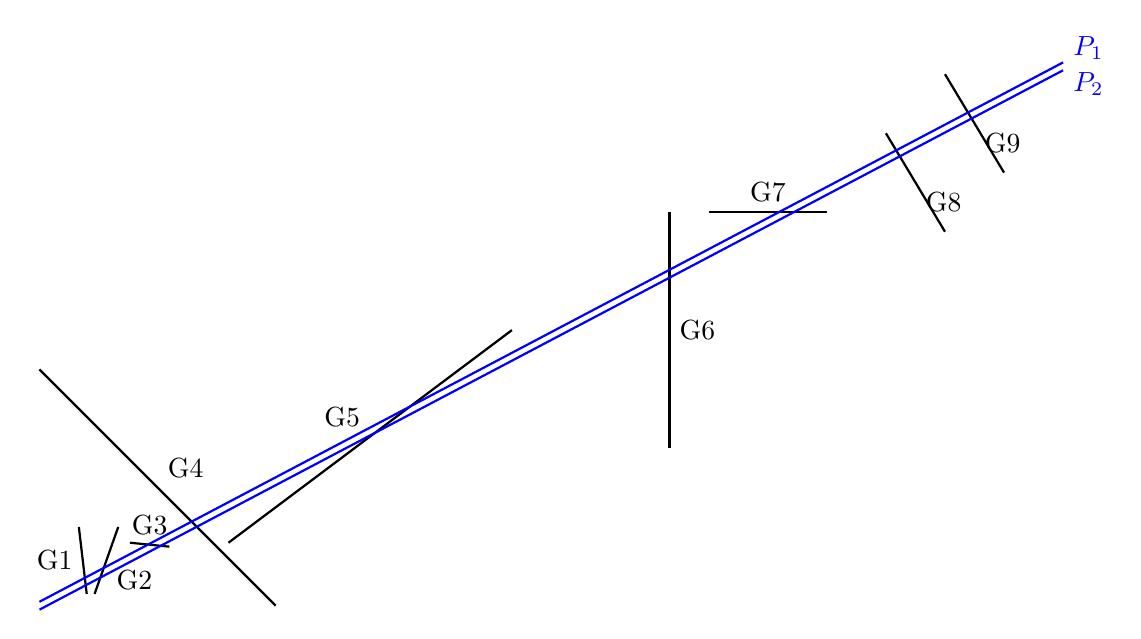
\begin{tikzpicture}[scale=1]

  \draw[thick] (0.5,1) -- (0.6,0.15) node[midway, left] {G1};

  \draw[thick] (1,1) -- (0.7,0.15) node[midway, below right] {G2};

  \draw[thick] (1.65,0.75) -- (1.15,0.8) node[midway, above] {G3};

  \draw[thick] (0,3) -- (3,0) node[midway, above right] {G4};

  \draw[thick] (2.4,0.8) -- (6,3.5) node[midway, above left] {G5};

  \draw[thick] (8,5) -- (8,2) node[midway, right] {G6};

  \draw[thick] (8.5,5) -- (10,5) node[midway, above] {G7};

  \draw[thick] (10.75,6) -- (11.5,4.75) node[midway, below right] {G8};

  \draw[thick] (11.5,6.75) -- (12.25,5.5) node[midway, below right] {G9};
  

\draw[thick, blue] (0,-0.05) -- (13,6.8) node[above right] {\(P_1\)};
\draw[thick, blue] (0,0.05) -- (13,6.9) node[below right] {\(P_2\)};
 
\end{tikzpicture}
\caption{Lösungsüberprüfung von zwei Parallelen.
Die Abbildung zeigt neun Torsegmente (\(G1\) bis \(G9\)). Außerdem sind zwei Parallelen \(P_1\) und \(P_2\) zu sehen. Sie stellen den Schusspfad des Balls dar. Da beide Parallelen einen Schnittpunkt mit jedem Tor besitzen ist dieser Schusspfad eine gültige Lösung.}
\end{figure}

Diese Schusspfadkonstruktion stellt damit den abschließenden Baustein des linearen Lösungsansatzes dar und ergänzt die zuvor beschriebenen Schritte zur Überprüfung der Tore sowie zur Filterung unwichtiger Pfosten. Dieser Algorithmus ermöglicht eine effiziente Lösung der Aufgabe 4 des 43. Bundeswettbewerbs Informatik.
